\documentclass[twoside]{book}

% Packages required by doxygen
\usepackage{fixltx2e}
\usepackage{calc}
\usepackage{doxygen}
\usepackage[export]{adjustbox} % also loads graphicx
\usepackage{graphicx}
\usepackage[utf8]{inputenc}
\usepackage{makeidx}
\usepackage{multicol}
\usepackage{multirow}
\PassOptionsToPackage{warn}{textcomp}
\usepackage{textcomp}
\usepackage[nointegrals]{wasysym}
\usepackage[table]{xcolor}

% Font selection
\usepackage[T1]{fontenc}
\usepackage[scaled=.90]{helvet}
\usepackage{courier}
\usepackage{amssymb}
\usepackage{sectsty}
\renewcommand{\familydefault}{\sfdefault}
\allsectionsfont{%
  \fontseries{bc}\selectfont%
  \color{darkgray}%
}
\renewcommand{\DoxyLabelFont}{%
  \fontseries{bc}\selectfont%
  \color{darkgray}%
}
\newcommand{\+}{\discretionary{\mbox{\scriptsize$\hookleftarrow$}}{}{}}

% Page & text layout
\usepackage{geometry}
\geometry{%
  a4paper,%
  top=2.5cm,%
  bottom=2.5cm,%
  left=2.5cm,%
  right=2.5cm%
}
\tolerance=750
\hfuzz=15pt
\hbadness=750
\setlength{\emergencystretch}{15pt}
\setlength{\parindent}{0cm}
\setlength{\parskip}{3ex plus 2ex minus 2ex}
\makeatletter
\renewcommand{\paragraph}{%
  \@startsection{paragraph}{4}{0ex}{-1.0ex}{1.0ex}{%
    \normalfont\normalsize\bfseries\SS@parafont%
  }%
}
\renewcommand{\subparagraph}{%
  \@startsection{subparagraph}{5}{0ex}{-1.0ex}{1.0ex}{%
    \normalfont\normalsize\bfseries\SS@subparafont%
  }%
}
\makeatother

% Headers & footers
\usepackage{fancyhdr}
\pagestyle{fancyplain}
\fancyhead[LE]{\fancyplain{}{\bfseries\thepage}}
\fancyhead[CE]{\fancyplain{}{}}
\fancyhead[RE]{\fancyplain{}{\bfseries\leftmark}}
\fancyhead[LO]{\fancyplain{}{\bfseries\rightmark}}
\fancyhead[CO]{\fancyplain{}{}}
\fancyhead[RO]{\fancyplain{}{\bfseries\thepage}}
\fancyfoot[LE]{\fancyplain{}{}}
\fancyfoot[CE]{\fancyplain{}{}}
\fancyfoot[RE]{\fancyplain{}{\bfseries\scriptsize Generated by Doxygen }}
\fancyfoot[LO]{\fancyplain{}{\bfseries\scriptsize Generated by Doxygen }}
\fancyfoot[CO]{\fancyplain{}{}}
\fancyfoot[RO]{\fancyplain{}{}}
\renewcommand{\footrulewidth}{0.4pt}
\renewcommand{\chaptermark}[1]{%
  \markboth{#1}{}%
}
\renewcommand{\sectionmark}[1]{%
  \markright{\thesection\ #1}%
}

% Indices & bibliography
\usepackage{natbib}
\usepackage[titles]{tocloft}
\setcounter{tocdepth}{3}
\setcounter{secnumdepth}{5}
\makeindex

% Hyperlinks (required, but should be loaded last)
\usepackage{ifpdf}
\ifpdf
  \usepackage[pdftex,pagebackref=true]{hyperref}
\else
  \usepackage[ps2pdf,pagebackref=true]{hyperref}
\fi
\hypersetup{%
  colorlinks=true,%
  linkcolor=blue,%
  citecolor=blue,%
  unicode%
}

% Custom commands
\newcommand{\clearemptydoublepage}{%
  \newpage{\pagestyle{empty}\cleardoublepage}%
}

\usepackage{caption}
\captionsetup{labelsep=space,justification=centering,font={bf},singlelinecheck=off,skip=4pt,position=top}

%===== C O N T E N T S =====

\begin{document}

% Titlepage & ToC
\hypersetup{pageanchor=false,
             bookmarksnumbered=true,
             pdfencoding=unicode
            }
\pagenumbering{roman}
\begin{titlepage}
\vspace*{7cm}
\begin{center}%
{\Large Reference Manual\\[1ex]\large 1.\+0 }\\
\vspace*{1cm}
{\large Generated by Doxygen 1.8.11}\\
\end{center}
\end{titlepage}
\clearemptydoublepage
\tableofcontents
\clearemptydoublepage
\pagenumbering{arabic}
\hypersetup{pageanchor=true}

%--- Begin generated contents ---
\chapter{G\+R\+E\+M\+L\+I\+NS (Gerenciador de Memória com Lista Encadeada Simples)}
\label{index}\hypertarget{index}{}\begin{DoxyAuthor}{Author}
Adelino Afonso Fernandes Avelino 

Irene Ginani Costa Pinheiro 
\end{DoxyAuthor}
\begin{DoxyDate}{Date}
Junho, 2016 
\end{DoxyDate}
\begin{DoxyVersion}{Version}
1.\+0 
\end{DoxyVersion}

\chapter{R\+E\+A\+D\+ME}
\label{md_README}
\hypertarget{md_README}{}
\#\+G\+R\+E\+M\+L\+I\+NS \subsubsection*{Ge\+R\+Enciador de Memoria com L\+Ista e\+Ncadeada Simples}

\subsection*{Descrição}

O G\+R\+E\+M\+L\+I\+NS é um gerenciador de memória que requisita ao sistema operacional um determinado bloco de memória e a partir do mesmo são realizadas operações de alocação de memória em blocos menores quando solicitado pelo cliente. No gremlins existem duas funções uma Allocate e uma Free nas quais uma realiza alocações e a outra libera memória alocada. Neste trabalho tivemos a colaboração do Professor Selan, na funcão de testes Storage\+Pool\+Test com o uso da priority\+\_\+queue a qual até então não estava sendo utilizada.

\subsection*{Compilação e execução}

{\bfseries Avaliando o Desempenho do GM} 
\begin{DoxyCode}
1 g++ -std=c++11 -pedantic -I include/ src/driver\_gremlins.cpp -o bin/exe && ./bin/exe
\end{DoxyCode}


{\bfseries Teste GM vs SO} 
\begin{DoxyCode}
1 g++ -std=c++11 -pedantic -I include/ src/drive\_comparador.cpp -o bin/exe && ./bin/exe 
\end{DoxyCode}


{\bfseries Teste de Allocate e Free} 
\begin{DoxyCode}
1 g++ -std=c++11 -pedantic -I include/ src/driver\_generico.cpp -o bin/exe -D TIPO1 && ./bin/exe
\end{DoxyCode}


{\bfseries Teste de Allocate Best e Free} 
\begin{DoxyCode}
1 g++ -std=c++11 -pedantic -I include/ src/driver\_generico.cpp -o bin/exe -D TIPO2 && ./bin/exe
\end{DoxyCode}
 \subsection*{Autores\+:}

Adelino Afonso Fernandes Avelino
\begin{DoxyItemize}
\item \href{https://github.com/aafavelino}{\tt Git\+Hub}
\end{DoxyItemize}

Irene Ginani Costa Pinheiro
\begin{DoxyItemize}
\item \href{https://github.com/IreneGinani}{\tt Git\+Hub}
\end{DoxyItemize}

\subsection*{Politica de colaboração}

{\bfseries Colaborador}

Selan R. dos Santos
\begin{DoxyItemize}
\item \href{https://www.dimap.ufrn.br/~selan/index.html}{\tt D\+I\+M\+Ap}
\end{DoxyItemize}

\subsection*{Disponível em\+:}

\href{https://github.com/aafavelino/GREMLINS}{\tt Projeto Gremlins} 
\chapter{Hierarchical Index}
\section{Class Hierarchy}
This inheritance list is sorted roughly, but not completely, alphabetically\+:\begin{DoxyCompactList}
\item \contentsline{section}{Event}{\pageref{class_event}}{}
\item \contentsline{section}{S\+L\+Pool\+:\+:Header}{\pageref{struct_s_l_pool_1_1_header}}{}
\begin{DoxyCompactList}
\item \contentsline{section}{S\+L\+Pool\+:\+:Block}{\pageref{struct_s_l_pool_1_1_block}}{}
\end{DoxyCompactList}
\item \contentsline{section}{Storage\+Pool}{\pageref{class_storage_pool}}{}
\begin{DoxyCompactList}
\item \contentsline{section}{S\+L\+Pool}{\pageref{class_s_l_pool}}{}
\end{DoxyCompactList}
\item \contentsline{section}{Tag}{\pageref{struct_tag}}{}
\end{DoxyCompactList}

\chapter{Class Index}
\section{Class List}
Here are the classes, structs, unions and interfaces with brief descriptions\+:\begin{DoxyCompactList}
\item\contentsline{section}{\hyperlink{struct_s_l_pool_1_1_block}{S\+L\+Pool\+::\+Block} \\*Struct \hyperlink{struct_s_l_pool_1_1_block}{Block} que define o tamanho em bytes do bloco de memória e ainda possui um ponteiro para o próximo e bloco }{\pageref{struct_s_l_pool_1_1_block}}{}
\item\contentsline{section}{\hyperlink{class_event}{Event} \\*Classe \hyperlink{class_event}{Event} }{\pageref{class_event}}{}
\item\contentsline{section}{\hyperlink{struct_s_l_pool_1_1_header}{S\+L\+Pool\+::\+Header} \\*Struct \hyperlink{struct_s_l_pool_1_1_header}{Header} com atributo do bloco }{\pageref{struct_s_l_pool_1_1_header}}{}
\item\contentsline{section}{\hyperlink{class_s_l_pool}{S\+L\+Pool} \\*Classe \hyperlink{class_s_l_pool}{S\+L\+Pool} }{\pageref{class_s_l_pool}}{}
\item\contentsline{section}{\hyperlink{class_storage_pool}{Storage\+Pool} }{\pageref{class_storage_pool}}{}
\item\contentsline{section}{\hyperlink{struct_tag}{Tag} \\*Struct tag que possui um roteiro do tipo \hyperlink{class_storage_pool}{Storage\+Pool} }{\pageref{struct_tag}}{}
\end{DoxyCompactList}

\chapter{File Index}
\section{File List}
Here is a list of all files with brief descriptions\+:\begin{DoxyCompactList}
\item\contentsline{section}{include/\hyperlink{_event_8h}{Event.\+h} \\*Corpo da Classe \hyperlink{class_event}{Event} }{\pageref{_event_8h}}{}
\item\contentsline{section}{include/\hyperlink{_event_8inl}{Event.\+inl} \\*Implementação da Classe \hyperlink{class_event}{Event} }{\pageref{_event_8inl}}{}
\item\contentsline{section}{include/\hyperlink{mempool__common_8h}{mempool\+\_\+common.\+h} }{\pageref{mempool__common_8h}}{}
\item\contentsline{section}{include/\hyperlink{mempool__common_8inl}{mempool\+\_\+common.\+inl} \\*Implementação do arquivo \hyperlink{mempool__common_8h}{mempool\+\_\+common.\+h} }{\pageref{mempool__common_8inl}}{}
\item\contentsline{section}{include/\hyperlink{_s_l_pool_8h}{S\+L\+Pool.\+h} \\*Assinatura da classe \hyperlink{class_s_l_pool}{S\+L\+Pool} }{\pageref{_s_l_pool_8h}}{}
\item\contentsline{section}{include/\hyperlink{_s_l_pool_8inl}{S\+L\+Pool.\+inl} \\*Implementação da Classe \hyperlink{class_s_l_pool}{S\+L\+Pool} }{\pageref{_s_l_pool_8inl}}{}
\item\contentsline{section}{include/\hyperlink{_storage_pool_8h}{Storage\+Pool.\+h} \\*Lista de métodos da classe abstrata \hyperlink{class_storage_pool}{Storage\+Pool} }{\pageref{_storage_pool_8h}}{}
\item\contentsline{section}{src/\hyperlink{drive__comparador_8cpp}{drive\+\_\+comparador.\+cpp} \\*Arquivo Main }{\pageref{drive__comparador_8cpp}}{}
\item\contentsline{section}{src/\hyperlink{driver__generico_8cpp}{driver\+\_\+generico.\+cpp} \\*Arquivo Main }{\pageref{driver__generico_8cpp}}{}
\item\contentsline{section}{src/\hyperlink{driver__gremlins_8cpp}{driver\+\_\+gremlins.\+cpp} \\*Arquivo Main }{\pageref{driver__gremlins_8cpp}}{}
\end{DoxyCompactList}

\chapter{Class Documentation}
\hypertarget{struct_s_l_pool_1_1_block}{}\section{S\+L\+Pool\+:\+:Block Struct Reference}
\label{struct_s_l_pool_1_1_block}\index{S\+L\+Pool\+::\+Block@{S\+L\+Pool\+::\+Block}}


struct \hyperlink{struct_s_l_pool_1_1_block}{Block} que define o tamanho em bytes do bloco de memória e ainda possui um ponteiro para o próximo e bloco.  




{\ttfamily \#include $<$S\+L\+Pool.\+h$>$}

Inheritance diagram for S\+L\+Pool\+:\+:Block\+:\begin{figure}[H]
\begin{center}
\leavevmode
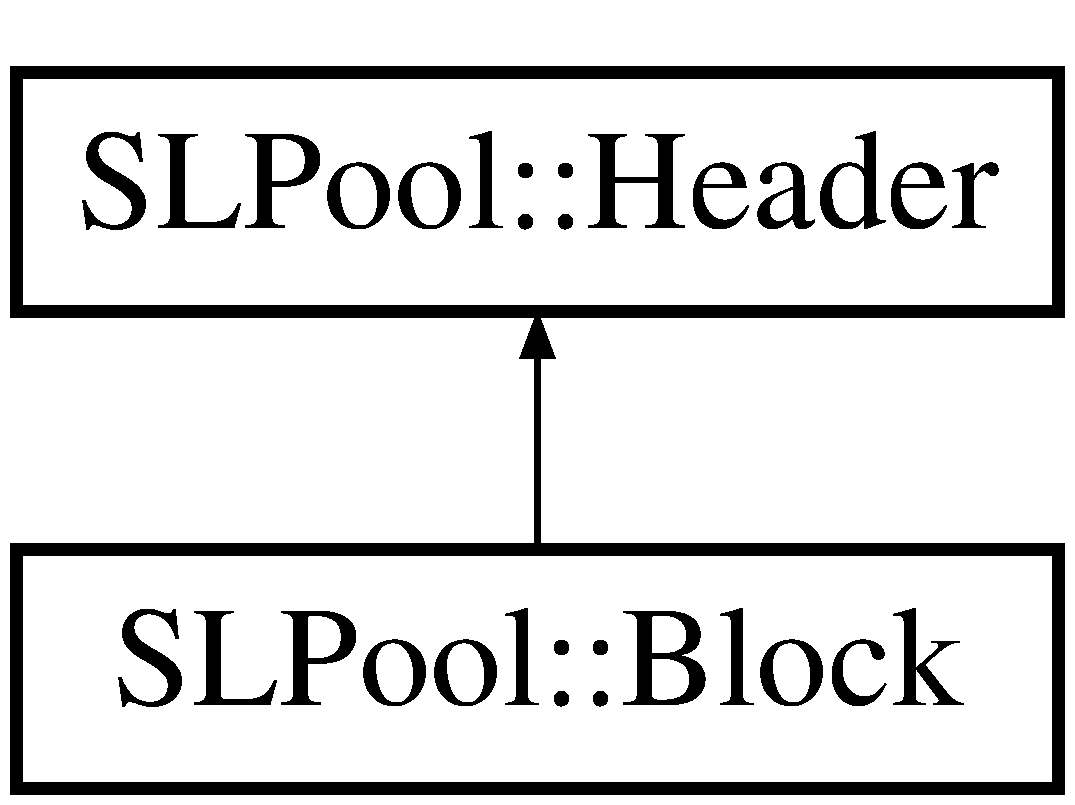
\includegraphics[height=2.000000cm]{struct_s_l_pool_1_1_block}
\end{center}
\end{figure}
\subsection*{Public Types}
\begin{DoxyCompactItemize}
\item 
enum \{ \hyperlink{struct_s_l_pool_1_1_block_adbb416e65dd0d7aa2121e30b34424db8a32fd11caed7c39eb5ab3949a612a14b9}{Block\+Size} = 16
 \}
\end{DoxyCompactItemize}
\subsection*{Public Member Functions}
\begin{DoxyCompactItemize}
\item 
\hyperlink{struct_s_l_pool_1_1_block_a2657816d1a41e84aa7ad25cdcf83ac60}{Block} ()
\end{DoxyCompactItemize}
\subsection*{Public Attributes}
\begin{DoxyCompactItemize}
\item 
\begin{tabbing}
xx\=xx\=xx\=xx\=xx\=xx\=xx\=xx\=xx\=\kill
union \{\\
\>\hyperlink{struct_s_l_pool_1_1_block}{Block} $\ast$ \hyperlink{struct_s_l_pool_1_1_block_ac626694affad2d9cdb8c93764d151225}{mp\_Next}\\
\>char \hyperlink{struct_s_l_pool_1_1_block_a5fcd86a9b213418deea8c65571290fbd}{mc\_RawArea} \mbox{[}\hyperlink{struct_s_l_pool_1_1_block_adbb416e65dd0d7aa2121e30b34424db8a32fd11caed7c39eb5ab3949a612a14b9}{BlockSize}-\/sizeof(\hyperlink{struct_s_l_pool_1_1_header}{Header})\mbox{]}\\
\}; \\

\end{tabbing}\end{DoxyCompactItemize}


\subsection{Detailed Description}
struct \hyperlink{struct_s_l_pool_1_1_block}{Block} que define o tamanho em bytes do bloco de memória e ainda possui um ponteiro para o próximo e bloco. 

\subsection{Member Enumeration Documentation}
\subsubsection[{\texorpdfstring{anonymous enum}{anonymous enum}}]{\setlength{\rightskip}{0pt plus 5cm}anonymous enum}\hypertarget{struct_s_l_pool_1_1_block_adbb416e65dd0d7aa2121e30b34424db8}{}\label{struct_s_l_pool_1_1_block_adbb416e65dd0d7aa2121e30b34424db8}
\begin{Desc}
\item[Enumerator]\par
\begin{description}
\index{Block\+Size@{Block\+Size}!S\+L\+Pool\+::\+Block@{S\+L\+Pool\+::\+Block}}\index{S\+L\+Pool\+::\+Block@{S\+L\+Pool\+::\+Block}!Block\+Size@{Block\+Size}}\item[{\em 
Block\+Size\hypertarget{struct_s_l_pool_1_1_block_adbb416e65dd0d7aa2121e30b34424db8a32fd11caed7c39eb5ab3949a612a14b9}{}\label{struct_s_l_pool_1_1_block_adbb416e65dd0d7aa2121e30b34424db8a32fd11caed7c39eb5ab3949a612a14b9}
}]\end{description}
\end{Desc}


\subsection{Constructor \& Destructor Documentation}
\index{S\+L\+Pool\+::\+Block@{S\+L\+Pool\+::\+Block}!Block@{Block}}
\index{Block@{Block}!S\+L\+Pool\+::\+Block@{S\+L\+Pool\+::\+Block}}
\subsubsection[{\texorpdfstring{Block()}{Block()}}]{\setlength{\rightskip}{0pt plus 5cm}S\+L\+Pool\+::\+Block\+::\+Block (
\begin{DoxyParamCaption}
{}
\end{DoxyParamCaption}
)\hspace{0.3cm}{\ttfamily [inline]}}\hypertarget{struct_s_l_pool_1_1_block_a2657816d1a41e84aa7ad25cdcf83ac60}{}\label{struct_s_l_pool_1_1_block_a2657816d1a41e84aa7ad25cdcf83ac60}


\subsection{Member Data Documentation}
\subsubsection[{\texorpdfstring{"@2}{@2}}]{\setlength{\rightskip}{0pt plus 5cm}union \{ ... \} }\hypertarget{struct_s_l_pool_1_1_block_a77176c27d7b62721129f2d2539ec72b5}{}\label{struct_s_l_pool_1_1_block_a77176c27d7b62721129f2d2539ec72b5}
\index{S\+L\+Pool\+::\+Block@{S\+L\+Pool\+::\+Block}!mc\+\_\+\+Raw\+Area@{mc\+\_\+\+Raw\+Area}}
\index{mc\+\_\+\+Raw\+Area@{mc\+\_\+\+Raw\+Area}!S\+L\+Pool\+::\+Block@{S\+L\+Pool\+::\+Block}}
\subsubsection[{\texorpdfstring{mc\+\_\+\+Raw\+Area}{mc_RawArea}}]{\setlength{\rightskip}{0pt plus 5cm}char S\+L\+Pool\+::\+Block\+::mc\+\_\+\+Raw\+Area\mbox{[}{\bf Block\+Size}-\/sizeof({\bf Header})\mbox{]}}\hypertarget{struct_s_l_pool_1_1_block_a5fcd86a9b213418deea8c65571290fbd}{}\label{struct_s_l_pool_1_1_block_a5fcd86a9b213418deea8c65571290fbd}
\index{S\+L\+Pool\+::\+Block@{S\+L\+Pool\+::\+Block}!mp\+\_\+\+Next@{mp\+\_\+\+Next}}
\index{mp\+\_\+\+Next@{mp\+\_\+\+Next}!S\+L\+Pool\+::\+Block@{S\+L\+Pool\+::\+Block}}
\subsubsection[{\texorpdfstring{mp\+\_\+\+Next}{mp_Next}}]{\setlength{\rightskip}{0pt plus 5cm}{\bf Block}$\ast$ S\+L\+Pool\+::\+Block\+::mp\+\_\+\+Next}\hypertarget{struct_s_l_pool_1_1_block_ac626694affad2d9cdb8c93764d151225}{}\label{struct_s_l_pool_1_1_block_ac626694affad2d9cdb8c93764d151225}


The documentation for this struct was generated from the following file\+:\begin{DoxyCompactItemize}
\item 
include/\hyperlink{_s_l_pool_8h}{S\+L\+Pool.\+h}\end{DoxyCompactItemize}

\hypertarget{class_event}{}\section{Event Class Reference}
\label{class_event}\index{Event@{Event}}


Classe \hyperlink{class_event}{Event}.  




{\ttfamily \#include $<$Event.\+h$>$}

\subsection*{Public Member Functions}
\begin{DoxyCompactItemize}
\item 
\hyperlink{class_event_aa4f1957692689f154f5f62f6c811dea2}{Event} (void $\ast$\+\_\+slave, std\+::time\+\_\+t \+\_\+time)
\begin{DoxyCompactList}\small\item\em Construtor da classe \hyperlink{class_event}{Event} Cria os \hyperlink{class_event}{Event}. \end{DoxyCompactList}\item 
\hyperlink{class_event_a5a40dd4708297f7031e29b39e039ae10}{Event} ()
\begin{DoxyCompactList}\small\item\em Construtor vazio da classe \hyperlink{class_event}{Event} Cria um evento vazio. \end{DoxyCompactList}\item 
void $\ast$ \hyperlink{class_event_a01de1d8ecbc8a0274b75822888cc8aad}{get\+\_\+slave} () const 
\begin{DoxyCompactList}\small\item\em recupera o valor do ponteiro void da classe \hyperlink{class_event}{Event} \end{DoxyCompactList}\item 
std\+::time\+\_\+t \hyperlink{class_event_a93534d78213f6bcb8651e6a8f11ed53a}{get\+\_\+time} () const 
\begin{DoxyCompactList}\small\item\em recupera o valor da variável time da classe \hyperlink{class_event}{Event} \end{DoxyCompactList}\item 
bool \hyperlink{class_event_a3e609dfa8eb5637d3ba9f7037c1927a9}{operator$<$} (\hyperlink{class_event}{Event} slave) const 
\begin{DoxyCompactList}\small\item\em redefine o operador $<$ \end{DoxyCompactList}\end{DoxyCompactItemize}


\subsection{Detailed Description}
Classe \hyperlink{class_event}{Event}. 

Assinaturas das funções e definição da classe \hyperlink{class_event}{Event} 

\subsection{Constructor \& Destructor Documentation}
\index{Event@{Event}!Event@{Event}}
\index{Event@{Event}!Event@{Event}}
\subsubsection[{\texorpdfstring{Event(void $\ast$\+\_\+slave, std\+::time\+\_\+t \+\_\+time)}{Event(void *_slave, std::time_t _time)}}]{\setlength{\rightskip}{0pt plus 5cm}Event\+::\+Event (
\begin{DoxyParamCaption}
\item[{void $\ast$}]{\+\_\+slave, }
\item[{std\+::time\+\_\+t}]{\+\_\+time}
\end{DoxyParamCaption}
)}\hypertarget{class_event_aa4f1957692689f154f5f62f6c811dea2}{}\label{class_event_aa4f1957692689f154f5f62f6c811dea2}


Construtor da classe \hyperlink{class_event}{Event} Cria os \hyperlink{class_event}{Event}. 

\index{Event@{Event}!Event@{Event}}
\index{Event@{Event}!Event@{Event}}
\subsubsection[{\texorpdfstring{Event()}{Event()}}]{\setlength{\rightskip}{0pt plus 5cm}Event\+::\+Event (
\begin{DoxyParamCaption}
{}
\end{DoxyParamCaption}
)\hspace{0.3cm}{\ttfamily [inline]}}\hypertarget{class_event_a5a40dd4708297f7031e29b39e039ae10}{}\label{class_event_a5a40dd4708297f7031e29b39e039ae10}


Construtor vazio da classe \hyperlink{class_event}{Event} Cria um evento vazio. 



\subsection{Member Function Documentation}
\index{Event@{Event}!get\+\_\+slave@{get\+\_\+slave}}
\index{get\+\_\+slave@{get\+\_\+slave}!Event@{Event}}
\subsubsection[{\texorpdfstring{get\+\_\+slave() const }{get_slave() const }}]{\setlength{\rightskip}{0pt plus 5cm}void $\ast$ Event\+::get\+\_\+slave (
\begin{DoxyParamCaption}
{}
\end{DoxyParamCaption}
) const}\hypertarget{class_event_a01de1d8ecbc8a0274b75822888cc8aad}{}\label{class_event_a01de1d8ecbc8a0274b75822888cc8aad}


recupera o valor do ponteiro void da classe \hyperlink{class_event}{Event} 

\begin{DoxyReturn}{Returns}
ponteiro void 
\end{DoxyReturn}
\index{Event@{Event}!get\+\_\+time@{get\+\_\+time}}
\index{get\+\_\+time@{get\+\_\+time}!Event@{Event}}
\subsubsection[{\texorpdfstring{get\+\_\+time() const }{get_time() const }}]{\setlength{\rightskip}{0pt plus 5cm}std\+::time\+\_\+t Event\+::get\+\_\+time (
\begin{DoxyParamCaption}
{}
\end{DoxyParamCaption}
) const}\hypertarget{class_event_a93534d78213f6bcb8651e6a8f11ed53a}{}\label{class_event_a93534d78213f6bcb8651e6a8f11ed53a}


recupera o valor da variável time da classe \hyperlink{class_event}{Event} 

\begin{DoxyReturn}{Returns}
time\+\_\+t 
\end{DoxyReturn}
\index{Event@{Event}!operator$<$@{operator$<$}}
\index{operator$<$@{operator$<$}!Event@{Event}}
\subsubsection[{\texorpdfstring{operator$<$(\+Event slave) const }{operator<(Event slave) const }}]{\setlength{\rightskip}{0pt plus 5cm}bool Event\+::operator$<$ (
\begin{DoxyParamCaption}
\item[{{\bf Event}}]{slave}
\end{DoxyParamCaption}
) const}\hypertarget{class_event_a3e609dfa8eb5637d3ba9f7037c1927a9}{}\label{class_event_a3e609dfa8eb5637d3ba9f7037c1927a9}


redefine o operador $<$ 


\begin{DoxyParams}{Parameters}
{\em salve} & parâmetro do tipo \hyperlink{class_event}{Event} utilizado pra comparação \\
\hline
\end{DoxyParams}
\begin{DoxyReturn}{Returns}
true ou false 
\end{DoxyReturn}


The documentation for this class was generated from the following files\+:\begin{DoxyCompactItemize}
\item 
include/\hyperlink{_event_8h}{Event.\+h}\item 
include/\hyperlink{_event_8inl}{Event.\+inl}\end{DoxyCompactItemize}

\hypertarget{struct_s_l_pool_1_1_header}{}\section{S\+L\+Pool\+:\+:Header Struct Reference}
\label{struct_s_l_pool_1_1_header}\index{S\+L\+Pool\+::\+Header@{S\+L\+Pool\+::\+Header}}


struct \hyperlink{struct_s_l_pool_1_1_header}{Header} com atributo do bloco  




{\ttfamily \#include $<$S\+L\+Pool.\+h$>$}

Inheritance diagram for S\+L\+Pool\+:\+:Header\+:\begin{figure}[H]
\begin{center}
\leavevmode
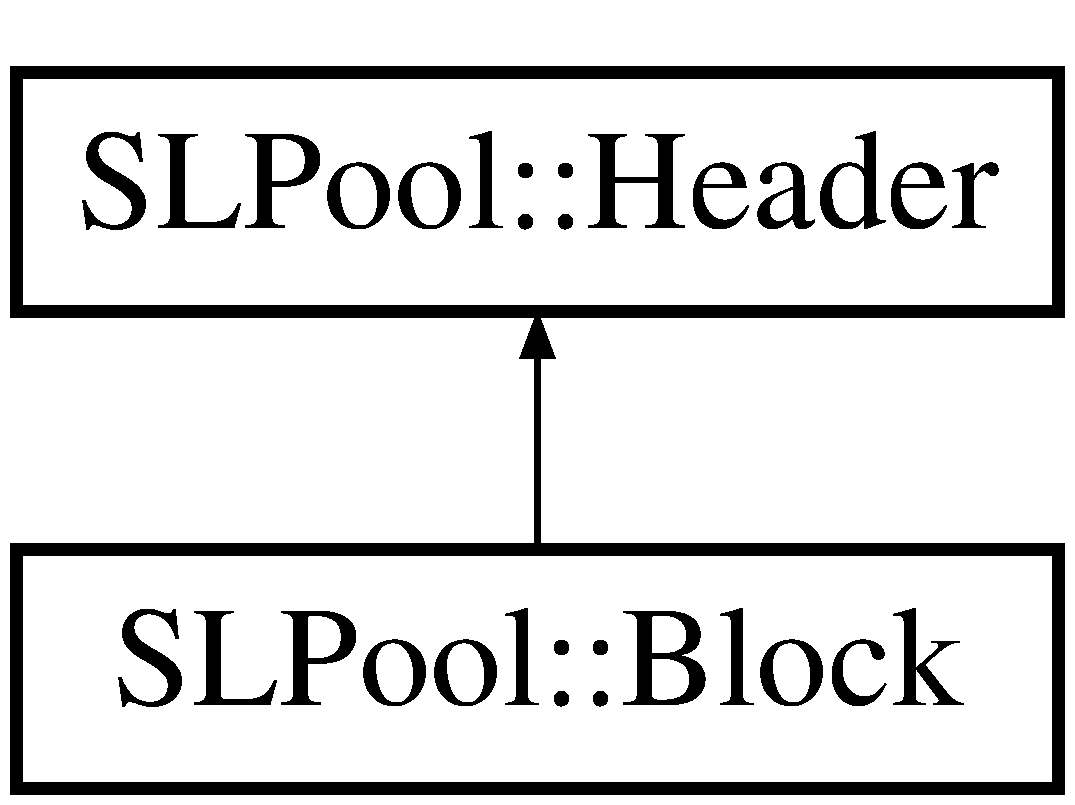
\includegraphics[height=2.000000cm]{struct_s_l_pool_1_1_header}
\end{center}
\end{figure}
\subsection*{Public Member Functions}
\begin{DoxyCompactItemize}
\item 
\hyperlink{struct_s_l_pool_1_1_header_af0a98001b684ebb3ca966a77f23b4d26}{Header} ()
\end{DoxyCompactItemize}
\subsection*{Public Attributes}
\begin{DoxyCompactItemize}
\item 
unsigned int \hyperlink{struct_s_l_pool_1_1_header_a0c06e96d58fa921e35411833364ad264}{mui\+\_\+\+Length}
\end{DoxyCompactItemize}


\subsection{Detailed Description}
struct \hyperlink{struct_s_l_pool_1_1_header}{Header} com atributo do bloco 

\subsection{Constructor \& Destructor Documentation}
\index{S\+L\+Pool\+::\+Header@{S\+L\+Pool\+::\+Header}!Header@{Header}}
\index{Header@{Header}!S\+L\+Pool\+::\+Header@{S\+L\+Pool\+::\+Header}}
\subsubsection[{\texorpdfstring{Header()}{Header()}}]{\setlength{\rightskip}{0pt plus 5cm}S\+L\+Pool\+::\+Header\+::\+Header (
\begin{DoxyParamCaption}
{}
\end{DoxyParamCaption}
)\hspace{0.3cm}{\ttfamily [inline]}}\hypertarget{struct_s_l_pool_1_1_header_af0a98001b684ebb3ca966a77f23b4d26}{}\label{struct_s_l_pool_1_1_header_af0a98001b684ebb3ca966a77f23b4d26}


\subsection{Member Data Documentation}
\index{S\+L\+Pool\+::\+Header@{S\+L\+Pool\+::\+Header}!mui\+\_\+\+Length@{mui\+\_\+\+Length}}
\index{mui\+\_\+\+Length@{mui\+\_\+\+Length}!S\+L\+Pool\+::\+Header@{S\+L\+Pool\+::\+Header}}
\subsubsection[{\texorpdfstring{mui\+\_\+\+Length}{mui_Length}}]{\setlength{\rightskip}{0pt plus 5cm}unsigned int S\+L\+Pool\+::\+Header\+::mui\+\_\+\+Length}\hypertarget{struct_s_l_pool_1_1_header_a0c06e96d58fa921e35411833364ad264}{}\label{struct_s_l_pool_1_1_header_a0c06e96d58fa921e35411833364ad264}


The documentation for this struct was generated from the following file\+:\begin{DoxyCompactItemize}
\item 
include/\hyperlink{_s_l_pool_8h}{S\+L\+Pool.\+h}\end{DoxyCompactItemize}

\hypertarget{class_s_l_pool}{}\section{S\+L\+Pool Class Reference}
\label{class_s_l_pool}\index{S\+L\+Pool@{S\+L\+Pool}}


Classe \hyperlink{class_s_l_pool}{S\+L\+Pool}.  




{\ttfamily \#include $<$S\+L\+Pool.\+h$>$}

Inheritance diagram for S\+L\+Pool\+:\begin{figure}[H]
\begin{center}
\leavevmode
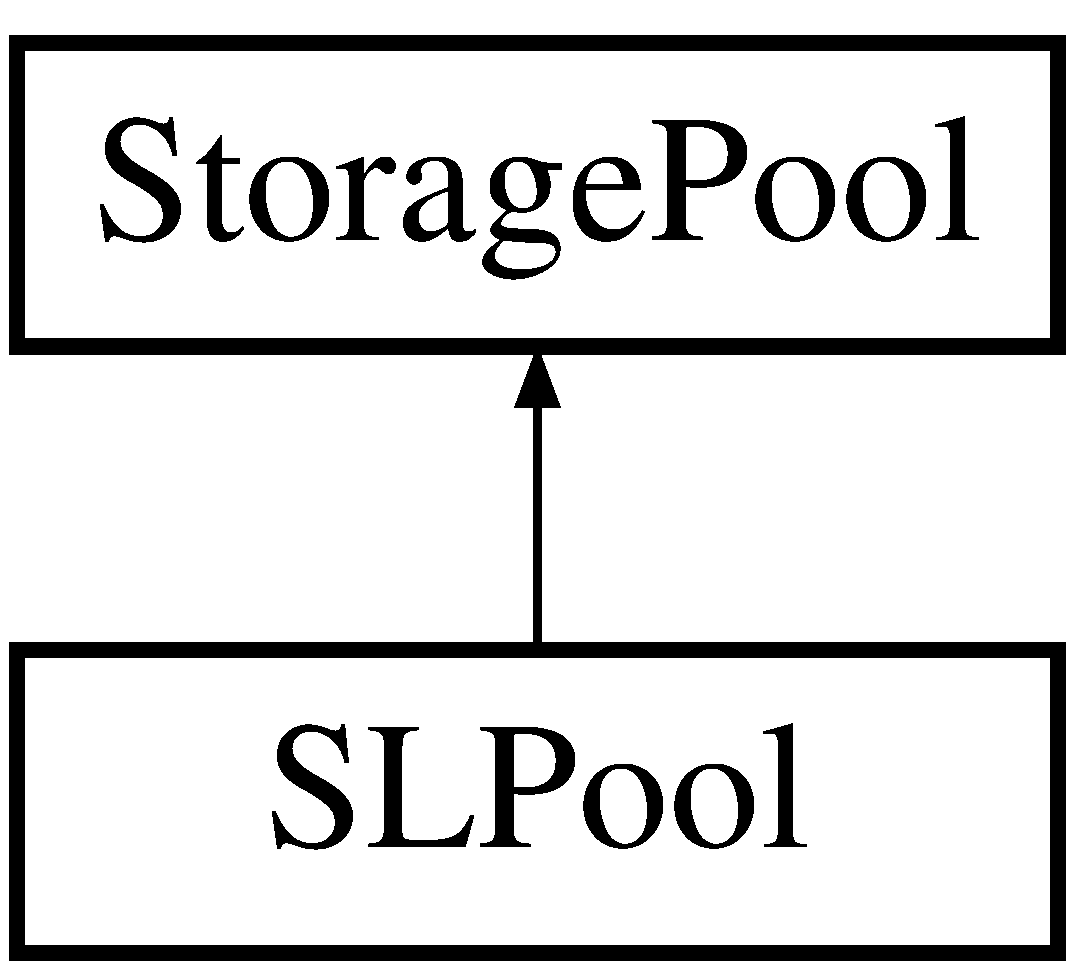
\includegraphics[height=2.000000cm]{class_s_l_pool}
\end{center}
\end{figure}
\subsection*{Classes}
\begin{DoxyCompactItemize}
\item 
struct \hyperlink{struct_s_l_pool_1_1_block}{Block}
\begin{DoxyCompactList}\small\item\em struct \hyperlink{struct_s_l_pool_1_1_block}{Block} que define o tamanho em bytes do bloco de memória e ainda possui um ponteiro para o próximo e bloco. \end{DoxyCompactList}\item 
struct \hyperlink{struct_s_l_pool_1_1_header}{Header}
\begin{DoxyCompactList}\small\item\em struct \hyperlink{struct_s_l_pool_1_1_header}{Header} com atributo do bloco \end{DoxyCompactList}\end{DoxyCompactItemize}
\subsection*{Public Member Functions}
\begin{DoxyCompactItemize}
\item 
\hyperlink{class_s_l_pool_aea29c4db7975b53f06c4fad1b5901cec}{S\+L\+Pool} (size\+\_\+t \+\_\+bytes)
\begin{DoxyCompactList}\small\item\em construtor da classe \hyperlink{class_s_l_pool}{S\+L\+Pool} \end{DoxyCompactList}\item 
virtual \hyperlink{class_s_l_pool_aec8dd0c2fe10addb1786447f8ed62c20}{$\sim$\+S\+L\+Pool} ()
\begin{DoxyCompactList}\small\item\em destrutor da classe \hyperlink{class_s_l_pool}{S\+L\+Pool} \end{DoxyCompactList}\item 
void $\ast$ \hyperlink{class_s_l_pool_a3bb05b3941f7e04113873ee57b8f3372}{Allocate} (size\+\_\+t bytes)
\begin{DoxyCompactList}\small\item\em método que aloca o valor passado por parâmetros no bloco inicial de memória seguinte o padrão first\+\_\+it \end{DoxyCompactList}\item 
void $\ast$ \hyperlink{class_s_l_pool_a67edac73b37d0252301591f73f3d4ecb}{Allocate\+\_\+best} (size\+\_\+t bytes)
\begin{DoxyCompactList}\small\item\em método que aloca o valor passado por parâmetros no bloco inicial de memória seguindo o padrão best\+\_\+it \end{DoxyCompactList}\item 
void \hyperlink{class_s_l_pool_aaa30890e07db032bf4834f832d4c5ac8}{Free} (void $\ast$ptr)
\begin{DoxyCompactList}\small\item\em método que libera o ponteiro passado como parâmetro \end{DoxyCompactList}\item 
void \hyperlink{class_s_l_pool_aafeaf06af67e80854ffbd9e9b5ad5f63}{Memory\+Map} (void)
\begin{DoxyCompactList}\small\item\em método que constrói um mapa da memória no momento atual \end{DoxyCompactList}\end{DoxyCompactItemize}


\subsection{Detailed Description}
Classe \hyperlink{class_s_l_pool}{S\+L\+Pool}. 

Assinaturas das funções e definição da classe \hyperlink{class_s_l_pool}{S\+L\+Pool} 

\subsection{Constructor \& Destructor Documentation}
\index{S\+L\+Pool@{S\+L\+Pool}!S\+L\+Pool@{S\+L\+Pool}}
\index{S\+L\+Pool@{S\+L\+Pool}!S\+L\+Pool@{S\+L\+Pool}}
\subsubsection[{\texorpdfstring{S\+L\+Pool(size\+\_\+t \+\_\+bytes)}{SLPool(size_t _bytes)}}]{\setlength{\rightskip}{0pt plus 5cm}S\+L\+Pool\+::\+S\+L\+Pool (
\begin{DoxyParamCaption}
\item[{size\+\_\+t}]{\+\_\+bytes}
\end{DoxyParamCaption}
)\hspace{0.3cm}{\ttfamily [explicit]}}\hypertarget{class_s_l_pool_aea29c4db7975b53f06c4fad1b5901cec}{}\label{class_s_l_pool_aea29c4db7975b53f06c4fad1b5901cec}


construtor da classe \hyperlink{class_s_l_pool}{S\+L\+Pool} 


\begin{DoxyParams}{Parameters}
{\em size\+\_\+t} & que constrói o primeiro bloco de memória do tamanho passado pelo parâmetro \\
\hline
\end{DoxyParams}
\index{S\+L\+Pool@{S\+L\+Pool}!````~S\+L\+Pool@{$\sim$\+S\+L\+Pool}}
\index{````~S\+L\+Pool@{$\sim$\+S\+L\+Pool}!S\+L\+Pool@{S\+L\+Pool}}
\subsubsection[{\texorpdfstring{$\sim$\+S\+L\+Pool()}{~SLPool()}}]{\setlength{\rightskip}{0pt plus 5cm}S\+L\+Pool\+::$\sim$\+S\+L\+Pool (
\begin{DoxyParamCaption}
{}
\end{DoxyParamCaption}
)\hspace{0.3cm}{\ttfamily [virtual]}}\hypertarget{class_s_l_pool_aec8dd0c2fe10addb1786447f8ed62c20}{}\label{class_s_l_pool_aec8dd0c2fe10addb1786447f8ed62c20}


destrutor da classe \hyperlink{class_s_l_pool}{S\+L\+Pool} 



\subsection{Member Function Documentation}
\index{S\+L\+Pool@{S\+L\+Pool}!Allocate@{Allocate}}
\index{Allocate@{Allocate}!S\+L\+Pool@{S\+L\+Pool}}
\subsubsection[{\texorpdfstring{Allocate(size\+\_\+t bytes)}{Allocate(size_t bytes)}}]{\setlength{\rightskip}{0pt plus 5cm}void $\ast$ S\+L\+Pool\+::\+Allocate (
\begin{DoxyParamCaption}
\item[{size\+\_\+t}]{bytes}
\end{DoxyParamCaption}
)\hspace{0.3cm}{\ttfamily [virtual]}}\hypertarget{class_s_l_pool_a3bb05b3941f7e04113873ee57b8f3372}{}\label{class_s_l_pool_a3bb05b3941f7e04113873ee57b8f3372}


método que aloca o valor passado por parâmetros no bloco inicial de memória seguinte o padrão first\+\_\+it 


\begin{DoxyParams}{Parameters}
{\em bytes} & em size\+\_\+t valor passado que se deseja alocar \\
\hline
\end{DoxyParams}
\begin{DoxyReturn}{Returns}
void 
\end{DoxyReturn}


Implements \hyperlink{class_storage_pool_a5de4eb49eafbf2adb86eb7e66739c947}{Storage\+Pool}.

\index{S\+L\+Pool@{S\+L\+Pool}!Allocate\+\_\+best@{Allocate\+\_\+best}}
\index{Allocate\+\_\+best@{Allocate\+\_\+best}!S\+L\+Pool@{S\+L\+Pool}}
\subsubsection[{\texorpdfstring{Allocate\+\_\+best(size\+\_\+t bytes)}{Allocate_best(size_t bytes)}}]{\setlength{\rightskip}{0pt plus 5cm}void $\ast$ S\+L\+Pool\+::\+Allocate\+\_\+best (
\begin{DoxyParamCaption}
\item[{size\+\_\+t}]{bytes}
\end{DoxyParamCaption}
)\hspace{0.3cm}{\ttfamily [virtual]}}\hypertarget{class_s_l_pool_a67edac73b37d0252301591f73f3d4ecb}{}\label{class_s_l_pool_a67edac73b37d0252301591f73f3d4ecb}


método que aloca o valor passado por parâmetros no bloco inicial de memória seguindo o padrão best\+\_\+it 


\begin{DoxyParams}{Parameters}
{\em bytes} & em size\+\_\+t valor passado que se deseja alocar \\
\hline
\end{DoxyParams}
\begin{DoxyReturn}{Returns}
void 
\end{DoxyReturn}


Implements \hyperlink{class_storage_pool_a9224f3fabf7ad7f5b80dd829ac30c69f}{Storage\+Pool}.

\index{S\+L\+Pool@{S\+L\+Pool}!Free@{Free}}
\index{Free@{Free}!S\+L\+Pool@{S\+L\+Pool}}
\subsubsection[{\texorpdfstring{Free(void $\ast$ptr)}{Free(void *ptr)}}]{\setlength{\rightskip}{0pt plus 5cm}void S\+L\+Pool\+::\+Free (
\begin{DoxyParamCaption}
\item[{void $\ast$}]{ptr}
\end{DoxyParamCaption}
)\hspace{0.3cm}{\ttfamily [virtual]}}\hypertarget{class_s_l_pool_aaa30890e07db032bf4834f832d4c5ac8}{}\label{class_s_l_pool_aaa30890e07db032bf4834f832d4c5ac8}


método que libera o ponteiro passado como parâmetro 


\begin{DoxyParams}{Parameters}
{\em ptr} & void que é o ponteiro o qual desejo liberar \\
\hline
\end{DoxyParams}
\begin{DoxyReturn}{Returns}
void 
\end{DoxyReturn}


Implements \hyperlink{class_storage_pool_a783b53d1799425318d9d4c3d5d90ac7c}{Storage\+Pool}.

\index{S\+L\+Pool@{S\+L\+Pool}!Memory\+Map@{Memory\+Map}}
\index{Memory\+Map@{Memory\+Map}!S\+L\+Pool@{S\+L\+Pool}}
\subsubsection[{\texorpdfstring{Memory\+Map(void)}{MemoryMap(void)}}]{\setlength{\rightskip}{0pt plus 5cm}void S\+L\+Pool\+::\+Memory\+Map (
\begin{DoxyParamCaption}
\item[{void}]{}
\end{DoxyParamCaption}
)\hspace{0.3cm}{\ttfamily [virtual]}}\hypertarget{class_s_l_pool_aafeaf06af67e80854ffbd9e9b5ad5f63}{}\label{class_s_l_pool_aafeaf06af67e80854ffbd9e9b5ad5f63}


método que constrói um mapa da memória no momento atual 

\begin{DoxyReturn}{Returns}
void 
\end{DoxyReturn}


Implements \hyperlink{class_storage_pool_aa30940ace73f59c81571feb4234abc1a}{Storage\+Pool}.



The documentation for this class was generated from the following files\+:\begin{DoxyCompactItemize}
\item 
include/\hyperlink{_s_l_pool_8h}{S\+L\+Pool.\+h}\item 
include/\hyperlink{_s_l_pool_8inl}{S\+L\+Pool.\+inl}\end{DoxyCompactItemize}

\hypertarget{class_storage_pool}{}\section{Storage\+Pool Class Reference}
\label{class_storage_pool}\index{Storage\+Pool@{Storage\+Pool}}


{\ttfamily \#include $<$Storage\+Pool.\+h$>$}

Inheritance diagram for Storage\+Pool\+:\begin{figure}[H]
\begin{center}
\leavevmode
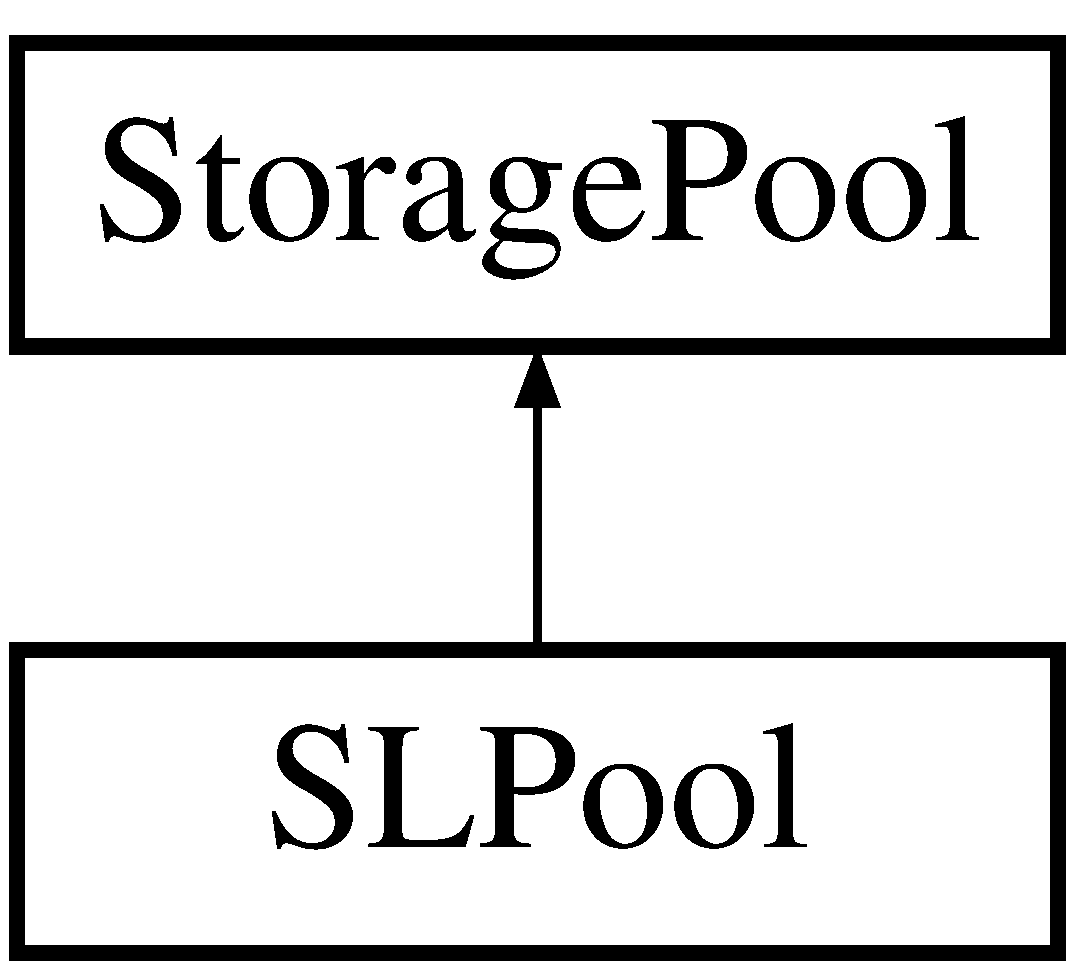
\includegraphics[height=2.000000cm]{class_storage_pool}
\end{center}
\end{figure}
\subsection*{Public Member Functions}
\begin{DoxyCompactItemize}
\item 
virtual \hyperlink{class_storage_pool_af762401e53c754fccb49703579bd3b31}{$\sim$\+Storage\+Pool} ()
\begin{DoxyCompactList}\small\item\em destrutor da classe \end{DoxyCompactList}\item 
virtual void $\ast$ \hyperlink{class_storage_pool_a5de4eb49eafbf2adb86eb7e66739c947}{Allocate} (size\+\_\+t bytes)=0
\begin{DoxyCompactList}\small\item\em método que aloca o valor passado por parâmetros no bloco inicial de memória seguinte o padrão first\+\_\+it \end{DoxyCompactList}\item 
virtual void $\ast$ \hyperlink{class_storage_pool_a9224f3fabf7ad7f5b80dd829ac30c69f}{Allocate\+\_\+best} (size\+\_\+t bytes)=0
\begin{DoxyCompactList}\small\item\em método que aloca o valor passado por parâmetros no bloco inicial de memória seguindo o padrão best\+\_\+it \end{DoxyCompactList}\item 
virtual void \hyperlink{class_storage_pool_a783b53d1799425318d9d4c3d5d90ac7c}{Free} (void $\ast$ptr)=0
\begin{DoxyCompactList}\small\item\em método que libera o ponteiro passado como parâmetro \end{DoxyCompactList}\item 
virtual void \hyperlink{class_storage_pool_aa30940ace73f59c81571feb4234abc1a}{Memory\+Map} (void)=0
\begin{DoxyCompactList}\small\item\em método que constrói um mapa da memória no momento atual \end{DoxyCompactList}\end{DoxyCompactItemize}


\subsection{Constructor \& Destructor Documentation}
\index{Storage\+Pool@{Storage\+Pool}!````~Storage\+Pool@{$\sim$\+Storage\+Pool}}
\index{````~Storage\+Pool@{$\sim$\+Storage\+Pool}!Storage\+Pool@{Storage\+Pool}}
\subsubsection[{\texorpdfstring{$\sim$\+Storage\+Pool()}{~StoragePool()}}]{\setlength{\rightskip}{0pt plus 5cm}virtual Storage\+Pool\+::$\sim$\+Storage\+Pool (
\begin{DoxyParamCaption}
{}
\end{DoxyParamCaption}
)\hspace{0.3cm}{\ttfamily [inline]}, {\ttfamily [virtual]}}\hypertarget{class_storage_pool_af762401e53c754fccb49703579bd3b31}{}\label{class_storage_pool_af762401e53c754fccb49703579bd3b31}


destrutor da classe 



\subsection{Member Function Documentation}
\index{Storage\+Pool@{Storage\+Pool}!Allocate@{Allocate}}
\index{Allocate@{Allocate}!Storage\+Pool@{Storage\+Pool}}
\subsubsection[{\texorpdfstring{Allocate(size\+\_\+t bytes)=0}{Allocate(size_t bytes)=0}}]{\setlength{\rightskip}{0pt plus 5cm}virtual void$\ast$ Storage\+Pool\+::\+Allocate (
\begin{DoxyParamCaption}
\item[{size\+\_\+t}]{bytes}
\end{DoxyParamCaption}
)\hspace{0.3cm}{\ttfamily [pure virtual]}}\hypertarget{class_storage_pool_a5de4eb49eafbf2adb86eb7e66739c947}{}\label{class_storage_pool_a5de4eb49eafbf2adb86eb7e66739c947}


método que aloca o valor passado por parâmetros no bloco inicial de memória seguinte o padrão first\+\_\+it 


\begin{DoxyParams}{Parameters}
{\em bytes} & em size\+\_\+t valor passado que se deseja alocar \\
\hline
\end{DoxyParams}
\begin{DoxyReturn}{Returns}
void 
\end{DoxyReturn}


Implemented in \hyperlink{class_s_l_pool_a3bb05b3941f7e04113873ee57b8f3372}{S\+L\+Pool}.

\index{Storage\+Pool@{Storage\+Pool}!Allocate\+\_\+best@{Allocate\+\_\+best}}
\index{Allocate\+\_\+best@{Allocate\+\_\+best}!Storage\+Pool@{Storage\+Pool}}
\subsubsection[{\texorpdfstring{Allocate\+\_\+best(size\+\_\+t bytes)=0}{Allocate_best(size_t bytes)=0}}]{\setlength{\rightskip}{0pt plus 5cm}virtual void$\ast$ Storage\+Pool\+::\+Allocate\+\_\+best (
\begin{DoxyParamCaption}
\item[{size\+\_\+t}]{bytes}
\end{DoxyParamCaption}
)\hspace{0.3cm}{\ttfamily [pure virtual]}}\hypertarget{class_storage_pool_a9224f3fabf7ad7f5b80dd829ac30c69f}{}\label{class_storage_pool_a9224f3fabf7ad7f5b80dd829ac30c69f}


método que aloca o valor passado por parâmetros no bloco inicial de memória seguindo o padrão best\+\_\+it 


\begin{DoxyParams}{Parameters}
{\em bytes} & em size\+\_\+t valor passado que se deseja alocar \\
\hline
\end{DoxyParams}
\begin{DoxyReturn}{Returns}
void 
\end{DoxyReturn}


Implemented in \hyperlink{class_s_l_pool_a67edac73b37d0252301591f73f3d4ecb}{S\+L\+Pool}.

\index{Storage\+Pool@{Storage\+Pool}!Free@{Free}}
\index{Free@{Free}!Storage\+Pool@{Storage\+Pool}}
\subsubsection[{\texorpdfstring{Free(void $\ast$ptr)=0}{Free(void *ptr)=0}}]{\setlength{\rightskip}{0pt plus 5cm}virtual void Storage\+Pool\+::\+Free (
\begin{DoxyParamCaption}
\item[{void $\ast$}]{ptr}
\end{DoxyParamCaption}
)\hspace{0.3cm}{\ttfamily [pure virtual]}}\hypertarget{class_storage_pool_a783b53d1799425318d9d4c3d5d90ac7c}{}\label{class_storage_pool_a783b53d1799425318d9d4c3d5d90ac7c}


método que libera o ponteiro passado como parâmetro 


\begin{DoxyParams}{Parameters}
{\em ptr} & void que é o ponteiro o qual desejo liberar \\
\hline
\end{DoxyParams}
\begin{DoxyReturn}{Returns}
void 
\end{DoxyReturn}


Implemented in \hyperlink{class_s_l_pool_aaa30890e07db032bf4834f832d4c5ac8}{S\+L\+Pool}.

\index{Storage\+Pool@{Storage\+Pool}!Memory\+Map@{Memory\+Map}}
\index{Memory\+Map@{Memory\+Map}!Storage\+Pool@{Storage\+Pool}}
\subsubsection[{\texorpdfstring{Memory\+Map(void)=0}{MemoryMap(void)=0}}]{\setlength{\rightskip}{0pt plus 5cm}virtual void Storage\+Pool\+::\+Memory\+Map (
\begin{DoxyParamCaption}
\item[{void}]{}
\end{DoxyParamCaption}
)\hspace{0.3cm}{\ttfamily [pure virtual]}}\hypertarget{class_storage_pool_aa30940ace73f59c81571feb4234abc1a}{}\label{class_storage_pool_aa30940ace73f59c81571feb4234abc1a}


método que constrói um mapa da memória no momento atual 

\begin{DoxyReturn}{Returns}
void 
\end{DoxyReturn}


Implemented in \hyperlink{class_s_l_pool_aafeaf06af67e80854ffbd9e9b5ad5f63}{S\+L\+Pool}.



The documentation for this class was generated from the following file\+:\begin{DoxyCompactItemize}
\item 
include/\hyperlink{_storage_pool_8h}{Storage\+Pool.\+h}\end{DoxyCompactItemize}

\hypertarget{struct_tag}{}\section{Tag Struct Reference}
\label{struct_tag}\index{Tag@{Tag}}


struct tag que possui um roteiro do tipo \hyperlink{class_storage_pool}{Storage\+Pool}  




{\ttfamily \#include $<$mempool\+\_\+common.\+h$>$}

\subsection*{Public Attributes}
\begin{DoxyCompactItemize}
\item 
\hyperlink{class_storage_pool}{Storage\+Pool} $\ast$ \hyperlink{struct_tag_aa4adbc74180401c6e0bff0a4c429f37e}{pool}
\end{DoxyCompactItemize}


\subsection{Detailed Description}
struct tag que possui um roteiro do tipo \hyperlink{class_storage_pool}{Storage\+Pool} 

\subsection{Member Data Documentation}
\index{Tag@{Tag}!pool@{pool}}
\index{pool@{pool}!Tag@{Tag}}
\subsubsection[{\texorpdfstring{pool}{pool}}]{\setlength{\rightskip}{0pt plus 5cm}{\bf Storage\+Pool}$\ast$ Tag\+::pool}\hypertarget{struct_tag_aa4adbc74180401c6e0bff0a4c429f37e}{}\label{struct_tag_aa4adbc74180401c6e0bff0a4c429f37e}


The documentation for this struct was generated from the following file\+:\begin{DoxyCompactItemize}
\item 
include/\hyperlink{mempool__common_8h}{mempool\+\_\+common.\+h}\end{DoxyCompactItemize}

\chapter{File Documentation}
\hypertarget{_event_8h}{}\section{include/\+Event.h File Reference}
\label{_event_8h}\index{include/\+Event.\+h@{include/\+Event.\+h}}


Corpo da Classe \hyperlink{class_event}{Event}.  


{\ttfamily \#include $<$ctime$>$}\\*
{\ttfamily \#include \char`\"{}Event.\+inl\char`\"{}}\\*
\subsection*{Classes}
\begin{DoxyCompactItemize}
\item 
class \hyperlink{class_event}{Event}
\begin{DoxyCompactList}\small\item\em Classe \hyperlink{class_event}{Event}. \end{DoxyCompactList}\end{DoxyCompactItemize}


\subsection{Detailed Description}
Corpo da Classe \hyperlink{class_event}{Event}. 

Arquivo com a classe \hyperlink{class_event}{Event} 
\hypertarget{_event_8inl}{}\section{include/\+Event.inl File Reference}
\label{_event_8inl}\index{include/\+Event.\+inl@{include/\+Event.\+inl}}


Implementação da Classe \hyperlink{class_event}{Event}.  


{\ttfamily \#include \char`\"{}Event.\+h\char`\"{}}\\*


\subsection{Detailed Description}
Implementação da Classe \hyperlink{class_event}{Event}. 

Arquivo com a construção das funções da classe \hyperlink{class_event}{Event} 
\hypertarget{mempool__common_8h}{}\section{include/mempool\+\_\+common.h File Reference}
\label{mempool__common_8h}\index{include/mempool\+\_\+common.\+h@{include/mempool\+\_\+common.\+h}}
{\ttfamily \#include $<$iostream$>$}\\*
{\ttfamily \#include \char`\"{}Storage\+Pool.\+h\char`\"{}}\\*
{\ttfamily \#include \char`\"{}mempool\+\_\+common.\+inl\char`\"{}}\\*
\subsection*{Classes}
\begin{DoxyCompactItemize}
\item 
struct \hyperlink{struct_tag}{Tag}
\begin{DoxyCompactList}\small\item\em struct tag que possui um roteiro do tipo \hyperlink{class_storage_pool}{Storage\+Pool} \end{DoxyCompactList}\end{DoxyCompactItemize}
\subsection*{Functions}
\begin{DoxyCompactItemize}
\item 
void $\ast$ \hyperlink{mempool__common_8h_ac5e850be5277fe21a0924d90adf671e6}{operator new} (size\+\_\+t bytes, \hyperlink{class_storage_pool}{Storage\+Pool} \&p)
\begin{DoxyCompactList}\small\item\em Sobrecarga do operador new. \end{DoxyCompactList}\item 
void $\ast$ \hyperlink{mempool__common_8h_a123745987bcf8adf0e5fa614a20c0137}{operator new} (size\+\_\+t bytes)
\begin{DoxyCompactList}\small\item\em Sobrecarga do operador new. \end{DoxyCompactList}\item 
void \hyperlink{mempool__common_8h_a49aeafb236d8e2fa3f1b687b6e0122db}{operator delete} (void $\ast$arg) noexcept
\begin{DoxyCompactList}\small\item\em Sobrecarga do operador delete. \end{DoxyCompactList}\item 
void $\ast$ \hyperlink{mempool__common_8h_a416a45bfcfcd41af3cb1caafca84761d}{operator new\mbox{[}$\,$\mbox{]}} (size\+\_\+t bytes, \hyperlink{class_storage_pool}{Storage\+Pool} \&p)
\begin{DoxyCompactList}\small\item\em Sobrecarga do operador new\mbox{[}\mbox{]}. \end{DoxyCompactList}\item 
void $\ast$ \hyperlink{mempool__common_8h_a9e317f35c05046679fe9434fb519068f}{operator new\mbox{[}$\,$\mbox{]}} (size\+\_\+t bytes)
\begin{DoxyCompactList}\small\item\em Sobrecarga do operador new\mbox{[}\mbox{]}. \end{DoxyCompactList}\end{DoxyCompactItemize}


\subsection{Function Documentation}
\index{mempool\+\_\+common.\+h@{mempool\+\_\+common.\+h}!operator delete@{operator delete}}
\index{operator delete@{operator delete}!mempool\+\_\+common.\+h@{mempool\+\_\+common.\+h}}
\subsubsection[{\texorpdfstring{operator delete(void $\ast$arg) noexcept}{operator delete(void *arg) noexcept}}]{\setlength{\rightskip}{0pt plus 5cm}void operator delete (
\begin{DoxyParamCaption}
\item[{void $\ast$}]{arg}
\end{DoxyParamCaption}
)\hspace{0.3cm}{\ttfamily [noexcept]}}\hypertarget{mempool__common_8h_a49aeafb236d8e2fa3f1b687b6e0122db}{}\label{mempool__common_8h_a49aeafb236d8e2fa3f1b687b6e0122db}


Sobrecarga do operador delete. 


\begin{DoxyParams}{Parameters}
{\em arg} & do tipo void utilizado para auxiliar destruir a memoria \\
\hline
\end{DoxyParams}
\index{mempool\+\_\+common.\+h@{mempool\+\_\+common.\+h}!operator new@{operator new}}
\index{operator new@{operator new}!mempool\+\_\+common.\+h@{mempool\+\_\+common.\+h}}
\subsubsection[{\texorpdfstring{operator new(size\+\_\+t bytes, Storage\+Pool \&p)}{operator new(size_t bytes, StoragePool &p)}}]{\setlength{\rightskip}{0pt plus 5cm}void$\ast$ operator new (
\begin{DoxyParamCaption}
\item[{size\+\_\+t}]{bytes, }
\item[{{\bf Storage\+Pool} \&}]{p}
\end{DoxyParamCaption}
)}\hypertarget{mempool__common_8h_ac5e850be5277fe21a0924d90adf671e6}{}\label{mempool__common_8h_ac5e850be5277fe21a0924d90adf671e6}


Sobrecarga do operador new. 


\begin{DoxyParams}{Parameters}
{\em bytes} & do tipo size\+\_\+t utilizado para calcular quanto é necessário alocar \\
\hline
{\em p} & do tipo \hyperlink{class_storage_pool}{Storage\+Pool} para ser utilizado como memória \\
\hline
\end{DoxyParams}
\index{mempool\+\_\+common.\+h@{mempool\+\_\+common.\+h}!operator new@{operator new}}
\index{operator new@{operator new}!mempool\+\_\+common.\+h@{mempool\+\_\+common.\+h}}
\subsubsection[{\texorpdfstring{operator new(size\+\_\+t bytes)}{operator new(size_t bytes)}}]{\setlength{\rightskip}{0pt plus 5cm}void$\ast$ operator new (
\begin{DoxyParamCaption}
\item[{size\+\_\+t}]{bytes}
\end{DoxyParamCaption}
)}\hypertarget{mempool__common_8h_a123745987bcf8adf0e5fa614a20c0137}{}\label{mempool__common_8h_a123745987bcf8adf0e5fa614a20c0137}


Sobrecarga do operador new. 


\begin{DoxyParams}{Parameters}
{\em bytes} & do tipo size\+\_\+t utilizado para calcular quanto é necessário alocar \\
\hline
\end{DoxyParams}
\index{mempool\+\_\+common.\+h@{mempool\+\_\+common.\+h}!operator new\mbox{[}$\,$\mbox{]}@{operator new[]}}
\index{operator new\mbox{[}$\,$\mbox{]}@{operator new[]}!mempool\+\_\+common.\+h@{mempool\+\_\+common.\+h}}
\subsubsection[{\texorpdfstring{operator new[](size\+\_\+t bytes, Storage\+Pool \&p)}{operator new[](size_t bytes, StoragePool &p)}}]{\setlength{\rightskip}{0pt plus 5cm}void$\ast$ operator new\mbox{[}$\,$\mbox{]} (
\begin{DoxyParamCaption}
\item[{size\+\_\+t}]{bytes, }
\item[{{\bf Storage\+Pool} \&}]{p}
\end{DoxyParamCaption}
)}\hypertarget{mempool__common_8h_a416a45bfcfcd41af3cb1caafca84761d}{}\label{mempool__common_8h_a416a45bfcfcd41af3cb1caafca84761d}


Sobrecarga do operador new\mbox{[}\mbox{]}. 


\begin{DoxyParams}{Parameters}
{\em bytes} & do tipo size\+\_\+t utilizado para calcular quanto é necessário alocar \\
\hline
{\em p} & do tipo \hyperlink{class_storage_pool}{Storage\+Pool} para ser utilizado como memória \\
\hline
\end{DoxyParams}
\index{mempool\+\_\+common.\+h@{mempool\+\_\+common.\+h}!operator new\mbox{[}$\,$\mbox{]}@{operator new[]}}
\index{operator new\mbox{[}$\,$\mbox{]}@{operator new[]}!mempool\+\_\+common.\+h@{mempool\+\_\+common.\+h}}
\subsubsection[{\texorpdfstring{operator new[](size\+\_\+t bytes)}{operator new[](size_t bytes)}}]{\setlength{\rightskip}{0pt plus 5cm}void$\ast$ operator new\mbox{[}$\,$\mbox{]} (
\begin{DoxyParamCaption}
\item[{size\+\_\+t}]{bytes}
\end{DoxyParamCaption}
)}\hypertarget{mempool__common_8h_a9e317f35c05046679fe9434fb519068f}{}\label{mempool__common_8h_a9e317f35c05046679fe9434fb519068f}


Sobrecarga do operador new\mbox{[}\mbox{]}. 


\begin{DoxyParams}{Parameters}
{\em bytes} & do tipo size\+\_\+t utilizado para calcular quanto é necessário alocar \\
\hline
\end{DoxyParams}

\hypertarget{mempool__common_8inl}{}\section{include/mempool\+\_\+common.inl File Reference}
\label{mempool__common_8inl}\index{include/mempool\+\_\+common.\+inl@{include/mempool\+\_\+common.\+inl}}


Implementação do arquivo \hyperlink{mempool__common_8h}{mempool\+\_\+common.\+h}.  


{\ttfamily \#include \char`\"{}mempool\+\_\+common.\+h\char`\"{}}\\*
{\ttfamily \#include \char`\"{}Storage\+Pool.\+h\char`\"{}}\\*
\subsection*{Functions}
\begin{DoxyCompactItemize}
\item 
void $\ast$ \hyperlink{mempool__common_8inl_ac5e850be5277fe21a0924d90adf671e6}{operator new} (size\+\_\+t bytes, \hyperlink{class_storage_pool}{Storage\+Pool} \&p)
\begin{DoxyCompactList}\small\item\em Sobrecarga do operador new. \end{DoxyCompactList}\item 
void $\ast$ \hyperlink{mempool__common_8inl_a123745987bcf8adf0e5fa614a20c0137}{operator new} (size\+\_\+t bytes)
\begin{DoxyCompactList}\small\item\em Sobrecarga do operador new. \end{DoxyCompactList}\item 
void $\ast$ \hyperlink{mempool__common_8inl_a416a45bfcfcd41af3cb1caafca84761d}{operator new\mbox{[}$\,$\mbox{]}} (size\+\_\+t bytes, \hyperlink{class_storage_pool}{Storage\+Pool} \&p)
\begin{DoxyCompactList}\small\item\em Sobrecarga do operador new\mbox{[}\mbox{]}. \end{DoxyCompactList}\item 
void $\ast$ \hyperlink{mempool__common_8inl_a9e317f35c05046679fe9434fb519068f}{operator new\mbox{[}$\,$\mbox{]}} (size\+\_\+t bytes)
\begin{DoxyCompactList}\small\item\em Sobrecarga do operador new\mbox{[}\mbox{]}. \end{DoxyCompactList}\item 
void \hyperlink{mempool__common_8inl_a49aeafb236d8e2fa3f1b687b6e0122db}{operator delete} (void $\ast$arg) noexcept
\begin{DoxyCompactList}\small\item\em Sobrecarga do operador delete. \end{DoxyCompactList}\end{DoxyCompactItemize}


\subsection{Detailed Description}
Implementação do arquivo \hyperlink{mempool__common_8h}{mempool\+\_\+common.\+h}. 



\subsection{Function Documentation}
\index{mempool\+\_\+common.\+inl@{mempool\+\_\+common.\+inl}!operator delete@{operator delete}}
\index{operator delete@{operator delete}!mempool\+\_\+common.\+inl@{mempool\+\_\+common.\+inl}}
\subsubsection[{\texorpdfstring{operator delete(void $\ast$arg) noexcept}{operator delete(void *arg) noexcept}}]{\setlength{\rightskip}{0pt plus 5cm}void operator delete (
\begin{DoxyParamCaption}
\item[{void $\ast$}]{arg}
\end{DoxyParamCaption}
)\hspace{0.3cm}{\ttfamily [noexcept]}}\hypertarget{mempool__common_8inl_a49aeafb236d8e2fa3f1b687b6e0122db}{}\label{mempool__common_8inl_a49aeafb236d8e2fa3f1b687b6e0122db}


Sobrecarga do operador delete. 


\begin{DoxyParams}{Parameters}
{\em arg} & do tipo void utilizado para auxiliar destruir a memoria \\
\hline
\end{DoxyParams}
\index{mempool\+\_\+common.\+inl@{mempool\+\_\+common.\+inl}!operator new@{operator new}}
\index{operator new@{operator new}!mempool\+\_\+common.\+inl@{mempool\+\_\+common.\+inl}}
\subsubsection[{\texorpdfstring{operator new(size\+\_\+t bytes, Storage\+Pool \&p)}{operator new(size_t bytes, StoragePool &p)}}]{\setlength{\rightskip}{0pt plus 5cm}void$\ast$ operator new (
\begin{DoxyParamCaption}
\item[{size\+\_\+t}]{bytes, }
\item[{{\bf Storage\+Pool} \&}]{p}
\end{DoxyParamCaption}
)}\hypertarget{mempool__common_8inl_ac5e850be5277fe21a0924d90adf671e6}{}\label{mempool__common_8inl_ac5e850be5277fe21a0924d90adf671e6}


Sobrecarga do operador new. 


\begin{DoxyParams}{Parameters}
{\em bytes} & do tipo size\+\_\+t utilizado para calcular quanto é necessário alocar \\
\hline
{\em p} & do tipo \hyperlink{class_storage_pool}{Storage\+Pool} para ser utilizado como memória \\
\hline
\end{DoxyParams}
\index{mempool\+\_\+common.\+inl@{mempool\+\_\+common.\+inl}!operator new@{operator new}}
\index{operator new@{operator new}!mempool\+\_\+common.\+inl@{mempool\+\_\+common.\+inl}}
\subsubsection[{\texorpdfstring{operator new(size\+\_\+t bytes)}{operator new(size_t bytes)}}]{\setlength{\rightskip}{0pt plus 5cm}void$\ast$ operator new (
\begin{DoxyParamCaption}
\item[{size\+\_\+t}]{bytes}
\end{DoxyParamCaption}
)}\hypertarget{mempool__common_8inl_a123745987bcf8adf0e5fa614a20c0137}{}\label{mempool__common_8inl_a123745987bcf8adf0e5fa614a20c0137}


Sobrecarga do operador new. 


\begin{DoxyParams}{Parameters}
{\em bytes} & do tipo size\+\_\+t utilizado para calcular quanto é necessário alocar \\
\hline
\end{DoxyParams}
\index{mempool\+\_\+common.\+inl@{mempool\+\_\+common.\+inl}!operator new\mbox{[}$\,$\mbox{]}@{operator new[]}}
\index{operator new\mbox{[}$\,$\mbox{]}@{operator new[]}!mempool\+\_\+common.\+inl@{mempool\+\_\+common.\+inl}}
\subsubsection[{\texorpdfstring{operator new[](size\+\_\+t bytes, Storage\+Pool \&p)}{operator new[](size_t bytes, StoragePool &p)}}]{\setlength{\rightskip}{0pt plus 5cm}void$\ast$ operator new\mbox{[}$\,$\mbox{]} (
\begin{DoxyParamCaption}
\item[{size\+\_\+t}]{bytes, }
\item[{{\bf Storage\+Pool} \&}]{p}
\end{DoxyParamCaption}
)}\hypertarget{mempool__common_8inl_a416a45bfcfcd41af3cb1caafca84761d}{}\label{mempool__common_8inl_a416a45bfcfcd41af3cb1caafca84761d}


Sobrecarga do operador new\mbox{[}\mbox{]}. 


\begin{DoxyParams}{Parameters}
{\em bytes} & do tipo size\+\_\+t utilizado para calcular quanto é necessário alocar \\
\hline
{\em p} & do tipo \hyperlink{class_storage_pool}{Storage\+Pool} para ser utilizado como memória \\
\hline
\end{DoxyParams}
\index{mempool\+\_\+common.\+inl@{mempool\+\_\+common.\+inl}!operator new\mbox{[}$\,$\mbox{]}@{operator new[]}}
\index{operator new\mbox{[}$\,$\mbox{]}@{operator new[]}!mempool\+\_\+common.\+inl@{mempool\+\_\+common.\+inl}}
\subsubsection[{\texorpdfstring{operator new[](size\+\_\+t bytes)}{operator new[](size_t bytes)}}]{\setlength{\rightskip}{0pt plus 5cm}void$\ast$ operator new\mbox{[}$\,$\mbox{]} (
\begin{DoxyParamCaption}
\item[{size\+\_\+t}]{bytes}
\end{DoxyParamCaption}
)}\hypertarget{mempool__common_8inl_a9e317f35c05046679fe9434fb519068f}{}\label{mempool__common_8inl_a9e317f35c05046679fe9434fb519068f}


Sobrecarga do operador new\mbox{[}\mbox{]}. 


\begin{DoxyParams}{Parameters}
{\em bytes} & do tipo size\+\_\+t utilizado para calcular quanto é necessário alocar \\
\hline
\end{DoxyParams}

\hypertarget{_s_l_pool_8h}{}\section{include/\+S\+L\+Pool.h File Reference}
\label{_s_l_pool_8h}\index{include/\+S\+L\+Pool.\+h@{include/\+S\+L\+Pool.\+h}}


Assinatura da classe \hyperlink{class_s_l_pool}{S\+L\+Pool}.  


{\ttfamily \#include $<$iostream$>$}\\*
{\ttfamily \#include $<$ctime$>$}\\*
{\ttfamily \#include $<$cmath$>$}\\*
{\ttfamily \#include $<$cstddef$>$}\\*
{\ttfamily \#include $<$cstdlib$>$}\\*
{\ttfamily \#include \char`\"{}Storage\+Pool.\+h\char`\"{}}\\*
{\ttfamily \#include \char`\"{}mempool\+\_\+common.\+h\char`\"{}}\\*
{\ttfamily \#include \char`\"{}S\+L\+Pool.\+inl\char`\"{}}\\*
\subsection*{Classes}
\begin{DoxyCompactItemize}
\item 
class \hyperlink{class_s_l_pool}{S\+L\+Pool}
\begin{DoxyCompactList}\small\item\em Classe \hyperlink{class_s_l_pool}{S\+L\+Pool}. \end{DoxyCompactList}\item 
struct \hyperlink{struct_s_l_pool_1_1_header}{S\+L\+Pool\+::\+Header}
\begin{DoxyCompactList}\small\item\em struct \hyperlink{struct_s_l_pool_1_1_header}{Header} com atributo do bloco \end{DoxyCompactList}\item 
struct \hyperlink{struct_s_l_pool_1_1_block}{S\+L\+Pool\+::\+Block}
\begin{DoxyCompactList}\small\item\em struct \hyperlink{struct_s_l_pool_1_1_block}{Block} que define o tamanho em bytes do bloco de memória e ainda possui um ponteiro para o próximo e bloco. \end{DoxyCompactList}\end{DoxyCompactItemize}


\subsection{Detailed Description}
Assinatura da classe \hyperlink{class_s_l_pool}{S\+L\+Pool}. 


\hypertarget{_s_l_pool_8inl}{}\section{include/\+S\+L\+Pool.inl File Reference}
\label{_s_l_pool_8inl}\index{include/\+S\+L\+Pool.\+inl@{include/\+S\+L\+Pool.\+inl}}


Implementação da Classe \hyperlink{class_s_l_pool}{S\+L\+Pool}.  


{\ttfamily \#include \char`\"{}S\+L\+Pool.\+h\char`\"{}}\\*


\subsection{Detailed Description}
Implementação da Classe \hyperlink{class_s_l_pool}{S\+L\+Pool}. 

Arquivo com a construção das funções da classe \hyperlink{class_s_l_pool}{S\+L\+Pool} 
\hypertarget{_storage_pool_8h}{}\section{include/\+Storage\+Pool.h File Reference}
\label{_storage_pool_8h}\index{include/\+Storage\+Pool.\+h@{include/\+Storage\+Pool.\+h}}


Lista de métodos da classe abstrata \hyperlink{class_storage_pool}{Storage\+Pool}.  


\subsection*{Classes}
\begin{DoxyCompactItemize}
\item 
class \hyperlink{class_storage_pool}{Storage\+Pool}
\end{DoxyCompactItemize}


\subsection{Detailed Description}
Lista de métodos da classe abstrata \hyperlink{class_storage_pool}{Storage\+Pool}. 


\hypertarget{_r_e_a_d_m_e_8md}{}\section{R\+E\+A\+D\+M\+E.\+md File Reference}
\label{_r_e_a_d_m_e_8md}\index{R\+E\+A\+D\+M\+E.\+md@{R\+E\+A\+D\+M\+E.\+md}}

\hypertarget{drive__comparador_8cpp}{}\section{src/drive\+\_\+comparador.cpp File Reference}
\label{drive__comparador_8cpp}\index{src/drive\+\_\+comparador.\+cpp@{src/drive\+\_\+comparador.\+cpp}}


Arquivo Main.  


{\ttfamily \#include $<$iostream$>$}\\*
{\ttfamily \#include $<$ctime$>$}\\*
{\ttfamily \#include $<$queue$>$}\\*
{\ttfamily \#include $<$chrono$>$}\\*
{\ttfamily \#include \char`\"{}mempool\+\_\+common.\+h\char`\"{}}\\*
{\ttfamily \#include \char`\"{}Event.\+h\char`\"{}}\\*
{\ttfamily \#include \char`\"{}S\+L\+Pool.\+h\char`\"{}}\\*
\subsection*{Functions}
\begin{DoxyCompactItemize}
\item 
void \hyperlink{drive__comparador_8cpp_a43e3ade1f50ae354cce63326d66c481d}{analise\+\_\+gm} ()
\begin{DoxyCompactList}\small\item\em Analise\+\_\+\+GM. \end{DoxyCompactList}\item 
void \hyperlink{drive__comparador_8cpp_a13552f70ddda8d9f7da0957c6a9ea4e8}{analise\+\_\+so} ()
\begin{DoxyCompactList}\small\item\em Analise\+\_\+\+SO. \end{DoxyCompactList}\item 
int \hyperlink{drive__comparador_8cpp_abf9e6b7e6f15df4b525a2e7705ba3089}{main} (int argc, char const $\ast$argv\mbox{[}$\,$\mbox{]})
\begin{DoxyCompactList}\small\item\em Main. \end{DoxyCompactList}\end{DoxyCompactItemize}


\subsection{Detailed Description}
Arquivo Main. 

Arquivo com o método Main 

\subsection{Function Documentation}
\index{drive\+\_\+comparador.\+cpp@{drive\+\_\+comparador.\+cpp}!analise\+\_\+gm@{analise\+\_\+gm}}
\index{analise\+\_\+gm@{analise\+\_\+gm}!drive\+\_\+comparador.\+cpp@{drive\+\_\+comparador.\+cpp}}
\subsubsection[{\texorpdfstring{analise\+\_\+gm()}{analise_gm()}}]{\setlength{\rightskip}{0pt plus 5cm}void analise\+\_\+gm (
\begin{DoxyParamCaption}
{}
\end{DoxyParamCaption}
)}\hypertarget{drive__comparador_8cpp_a43e3ade1f50ae354cce63326d66c481d}{}\label{drive__comparador_8cpp_a43e3ade1f50ae354cce63326d66c481d}


Analise\+\_\+\+GM. 

Utilização das sobrecargas dos operadores new e delete \index{drive\+\_\+comparador.\+cpp@{drive\+\_\+comparador.\+cpp}!analise\+\_\+so@{analise\+\_\+so}}
\index{analise\+\_\+so@{analise\+\_\+so}!drive\+\_\+comparador.\+cpp@{drive\+\_\+comparador.\+cpp}}
\subsubsection[{\texorpdfstring{analise\+\_\+so()}{analise_so()}}]{\setlength{\rightskip}{0pt plus 5cm}void analise\+\_\+so (
\begin{DoxyParamCaption}
{}
\end{DoxyParamCaption}
)}\hypertarget{drive__comparador_8cpp_a13552f70ddda8d9f7da0957c6a9ea4e8}{}\label{drive__comparador_8cpp_a13552f70ddda8d9f7da0957c6a9ea4e8}


Analise\+\_\+\+SO. 

Utilização dos operadores new e delete do sistema \index{drive\+\_\+comparador.\+cpp@{drive\+\_\+comparador.\+cpp}!main@{main}}
\index{main@{main}!drive\+\_\+comparador.\+cpp@{drive\+\_\+comparador.\+cpp}}
\subsubsection[{\texorpdfstring{main(int argc, char const $\ast$argv[])}{main(int argc, char const *argv[])}}]{\setlength{\rightskip}{0pt plus 5cm}int main (
\begin{DoxyParamCaption}
\item[{int}]{argc, }
\item[{char const $\ast$}]{argv\mbox{[}$\,$\mbox{]}}
\end{DoxyParamCaption}
)}\hypertarget{drive__comparador_8cpp_abf9e6b7e6f15df4b525a2e7705ba3089}{}\label{drive__comparador_8cpp_abf9e6b7e6f15df4b525a2e7705ba3089}


Main. 

Drive do programa que compara o gerenciador desenvolvido com o do SO 
\hypertarget{driver__generico_8cpp}{}\section{src/driver\+\_\+generico.cpp File Reference}
\label{driver__generico_8cpp}\index{src/driver\+\_\+generico.\+cpp@{src/driver\+\_\+generico.\+cpp}}


Arquivo Main.  


{\ttfamily \#include $<$iostream$>$}\\*
{\ttfamily \#include $<$ctime$>$}\\*
{\ttfamily \#include $<$queue$>$}\\*
{\ttfamily \#include \char`\"{}mempool\+\_\+common.\+h\char`\"{}}\\*
{\ttfamily \#include \char`\"{}Event.\+h\char`\"{}}\\*
{\ttfamily \#include \char`\"{}S\+L\+Pool.\+h\char`\"{}}\\*
\subsection*{Functions}
\begin{DoxyCompactItemize}
\item 
int \hyperlink{driver__generico_8cpp_abf9e6b7e6f15df4b525a2e7705ba3089}{main} (int argc, char const $\ast$argv\mbox{[}$\,$\mbox{]})
\begin{DoxyCompactList}\small\item\em Main. \end{DoxyCompactList}\end{DoxyCompactItemize}


\subsection{Detailed Description}
Arquivo Main. 

Arquivo com o método Main 

\subsection{Function Documentation}
\index{driver\+\_\+generico.\+cpp@{driver\+\_\+generico.\+cpp}!main@{main}}
\index{main@{main}!driver\+\_\+generico.\+cpp@{driver\+\_\+generico.\+cpp}}
\subsubsection[{\texorpdfstring{main(int argc, char const $\ast$argv[])}{main(int argc, char const *argv[])}}]{\setlength{\rightskip}{0pt plus 5cm}int main (
\begin{DoxyParamCaption}
\item[{int}]{argc, }
\item[{char const $\ast$}]{argv\mbox{[}$\,$\mbox{]}}
\end{DoxyParamCaption}
)}\hypertarget{driver__generico_8cpp_abf9e6b7e6f15df4b525a2e7705ba3089}{}\label{driver__generico_8cpp_abf9e6b7e6f15df4b525a2e7705ba3089}


Main. 

Teste genérico para utilizar de maneira básica as funções de alocação e liberação de memória 
\hypertarget{driver__gremlins_8cpp}{}\section{src/driver\+\_\+gremlins.cpp File Reference}
\label{driver__gremlins_8cpp}\index{src/driver\+\_\+gremlins.\+cpp@{src/driver\+\_\+gremlins.\+cpp}}


Arquivo Main.  


{\ttfamily \#include $<$iostream$>$}\\*
{\ttfamily \#include $<$ctime$>$}\\*
{\ttfamily \#include $<$chrono$>$}\\*
{\ttfamily \#include $<$queue$>$}\\*
{\ttfamily \#include $<$vector$>$}\\*
{\ttfamily \#include \char`\"{}mempool\+\_\+common.\+h\char`\"{}}\\*
{\ttfamily \#include \char`\"{}Event.\+h\char`\"{}}\\*
{\ttfamily \#include \char`\"{}S\+L\+Pool.\+h\char`\"{}}\\*
\subsection*{Functions}
\begin{DoxyCompactItemize}
\item 
void \hyperlink{driver__gremlins_8cpp_a16089dc62e25d124a9557c76c5f472c8}{Storage\+Pool\+Test} (\hyperlink{class_storage_pool}{Storage\+Pool} $\ast$pool, size\+\_\+t \+\_\+time\+Limit)
\item 
int \hyperlink{driver__gremlins_8cpp_abf9e6b7e6f15df4b525a2e7705ba3089}{main} (int argc, char const $\ast$argv\mbox{[}$\,$\mbox{]})
\begin{DoxyCompactList}\small\item\em Main. \end{DoxyCompactList}\end{DoxyCompactItemize}


\subsection{Detailed Description}
Arquivo Main. 

Arquivo com o método Main 

\subsection{Function Documentation}
\index{driver\+\_\+gremlins.\+cpp@{driver\+\_\+gremlins.\+cpp}!main@{main}}
\index{main@{main}!driver\+\_\+gremlins.\+cpp@{driver\+\_\+gremlins.\+cpp}}
\subsubsection[{\texorpdfstring{main(int argc, char const $\ast$argv[])}{main(int argc, char const *argv[])}}]{\setlength{\rightskip}{0pt plus 5cm}int main (
\begin{DoxyParamCaption}
\item[{int}]{argc, }
\item[{char const $\ast$}]{argv\mbox{[}$\,$\mbox{]}}
\end{DoxyParamCaption}
)}\hypertarget{driver__gremlins_8cpp_abf9e6b7e6f15df4b525a2e7705ba3089}{}\label{driver__gremlins_8cpp_abf9e6b7e6f15df4b525a2e7705ba3089}


Main. 

Teste sugerido para comprovar eficiencia do GM desenvolvido \index{driver\+\_\+gremlins.\+cpp@{driver\+\_\+gremlins.\+cpp}!Storage\+Pool\+Test@{Storage\+Pool\+Test}}
\index{Storage\+Pool\+Test@{Storage\+Pool\+Test}!driver\+\_\+gremlins.\+cpp@{driver\+\_\+gremlins.\+cpp}}
\subsubsection[{\texorpdfstring{Storage\+Pool\+Test(\+Storage\+Pool $\ast$pool, size\+\_\+t \+\_\+time\+Limit)}{StoragePoolTest(StoragePool *pool, size_t _timeLimit)}}]{\setlength{\rightskip}{0pt plus 5cm}void Storage\+Pool\+Test (
\begin{DoxyParamCaption}
\item[{{\bf Storage\+Pool} $\ast$}]{pool, }
\item[{size\+\_\+t}]{\+\_\+time\+Limit}
\end{DoxyParamCaption}
)}\hypertarget{driver__gremlins_8cpp_a16089dc62e25d124a9557c76c5f472c8}{}\label{driver__gremlins_8cpp_a16089dc62e25d124a9557c76c5f472c8}

%--- End generated contents ---

% Index
\backmatter
\newpage
\phantomsection
\clearemptydoublepage
\addcontentsline{toc}{chapter}{Index}
\printindex

\end{document}
